这里讨论的模式是McCool等人在《结构化并行编程》一书中描述并行模式的子集。我们不讨论与并行性类型相关的模式(例如fork-join、分支绑定),而是关注对编写数据并行内核最有用的算法模式。\par

理解并行模式的这个子集对于成为一个高效的DPC++程序员至关重要。图14-1中的表给出了不同模式的概述,包括主要用例、关键属性,以及属性如何影响不同硬件设备的亲和性。\par

\hspace*{\fill} \par %插入空行
图14-1 并行模式及其对不同设备类型的亲和性
\begin{table}[H]
	\begin{tabular}{|l|l|l|l|}
		\hline
		\textbf{模式}                                           & \textbf{用于}                                                        & \textbf{关键属性}                                                            & \textbf{设备亲和度}                                          \\ \hline
		Map                                                        & \begin{tabular}[c]{@{}l@{}}简单的并行内核\end{tabular}          & \begin{tabular}[c]{@{}l@{}}无数据依赖性和高可扩展性\end{tabular} & 所有设备                                                               \\ \hline
		Stencil                                                    & \begin{tabular}[c]{@{}l@{}}结构化数据依赖性\end{tabular}      & \begin{tabular}[c]{@{}l@{}}数据依赖和数据重用\end{tabular}         & \begin{tabular}[c]{@{}l@{}}取决于模具的大小\end{tabular} \\ \hline
		Reduction                                                  & \begin{tabular}[c]{@{}l@{}}合并部分结果\end{tabular}        & 数据依赖                                                                   & 所有设备                                                                \\ \hline
		\begin{tabular}[c]{@{}l@{}}Scan\\ Pack/Unpack\end{tabular} & \begin{tabular}[c]{@{}l@{}}筛选和重组数据\end{tabular} & 有限的可扩展性                                                                & \begin{tabular}[c]{@{}l@{}}取决于问题的大小\end{tabular} \\ \hline
	\end{tabular}
\end{table}

\hspace*{\fill} \par %插入空行
\textbf{Map——映射}

映射模式是所有并行模式中最简单的,具有函数式编程语言经验的读者很快就会熟悉它。如图14-2所示,范围内的每个输入元素通过应用某个函数独立映射到一个输出。许多数据并行操作可以表示为映射模式(例如,向量加法)。\par

\hspace*{\fill} \par %插入空行
图14-2 映射模式
\begin{center}
	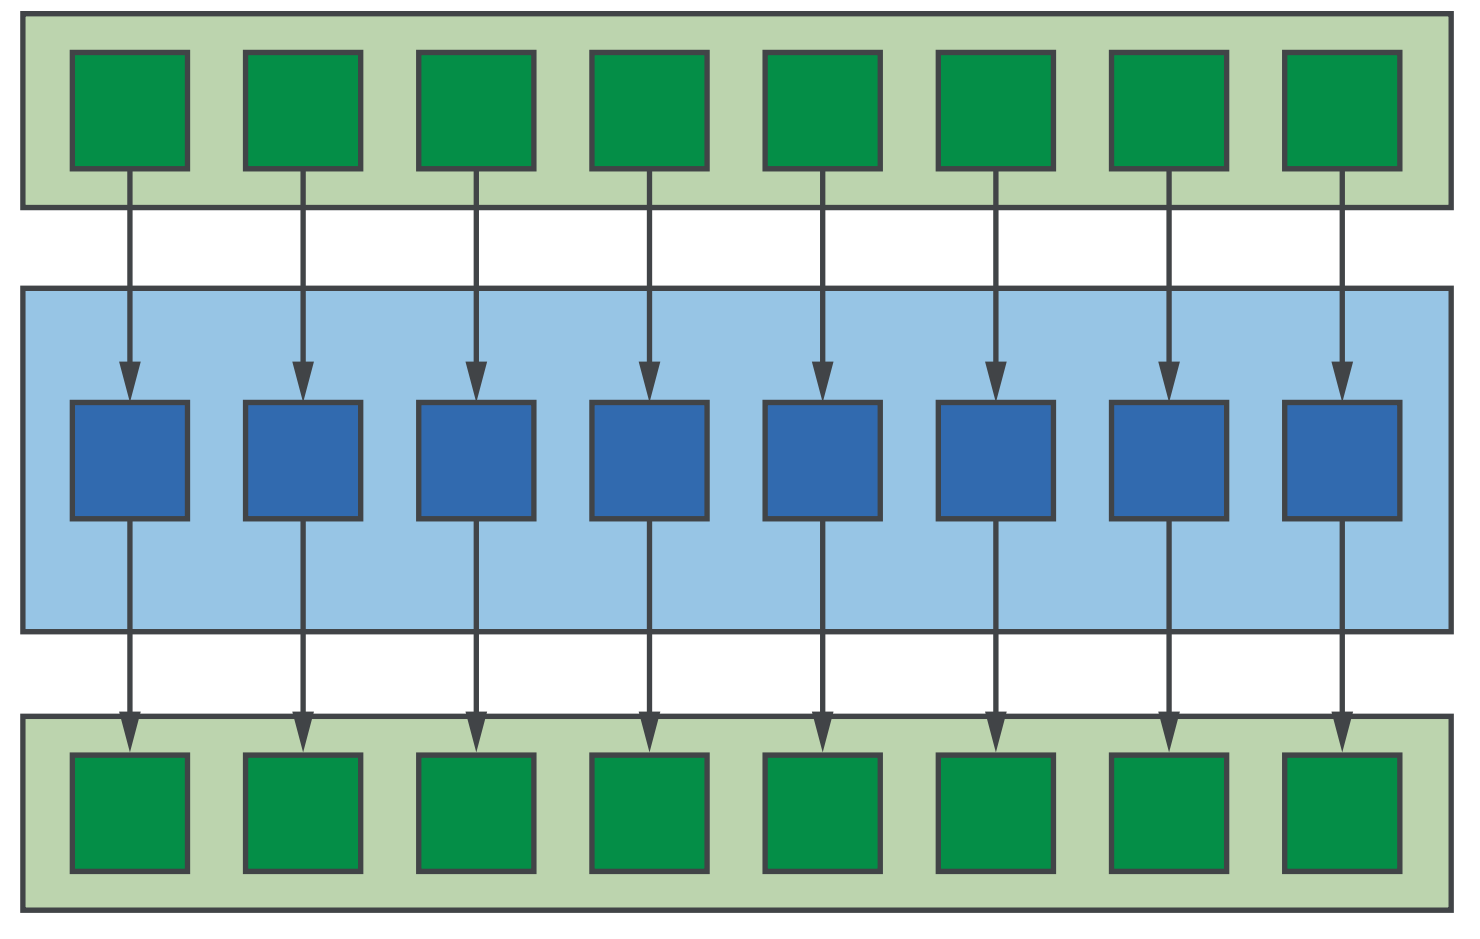
\includegraphics[width=1.\textwidth]{content/chapter-14/images/2}
\end{center}

由于每个应用程序的函数都完全独立,所以映射的表达式通常非常简单,依赖于编译器和/或运行时来做大部分工作。写入映射模式的内核应该能够适用于任何设备,并且这些内核的性能能根据可用的硬件并行度进行很好地扩展。\par

然而,在决定将整个应用程序重写为一系列映射内核之前,应该仔细考虑!这样的开发方法是高效的,保证了应用程序可以移植到各种设备类型,但却忽略那些可能显著提高性能的优化(例如,数据重用,融合内核)。\par

\hspace*{\fill} \par %插入空行
\textbf{Stencil——模具}

模具模式与映射模式密切相关。如图14-3所示,一个函数应用到一个输入和一组由模板描述的邻近输入,以产生单个输出。模板模式经常出现在许多领域,包括科学/工程应用(如有限差分)和计算机视觉/机器学习应用(如图像卷积)。\par

\hspace*{\fill} \par %插入空行
图14-3 模具模式
\begin{center}
	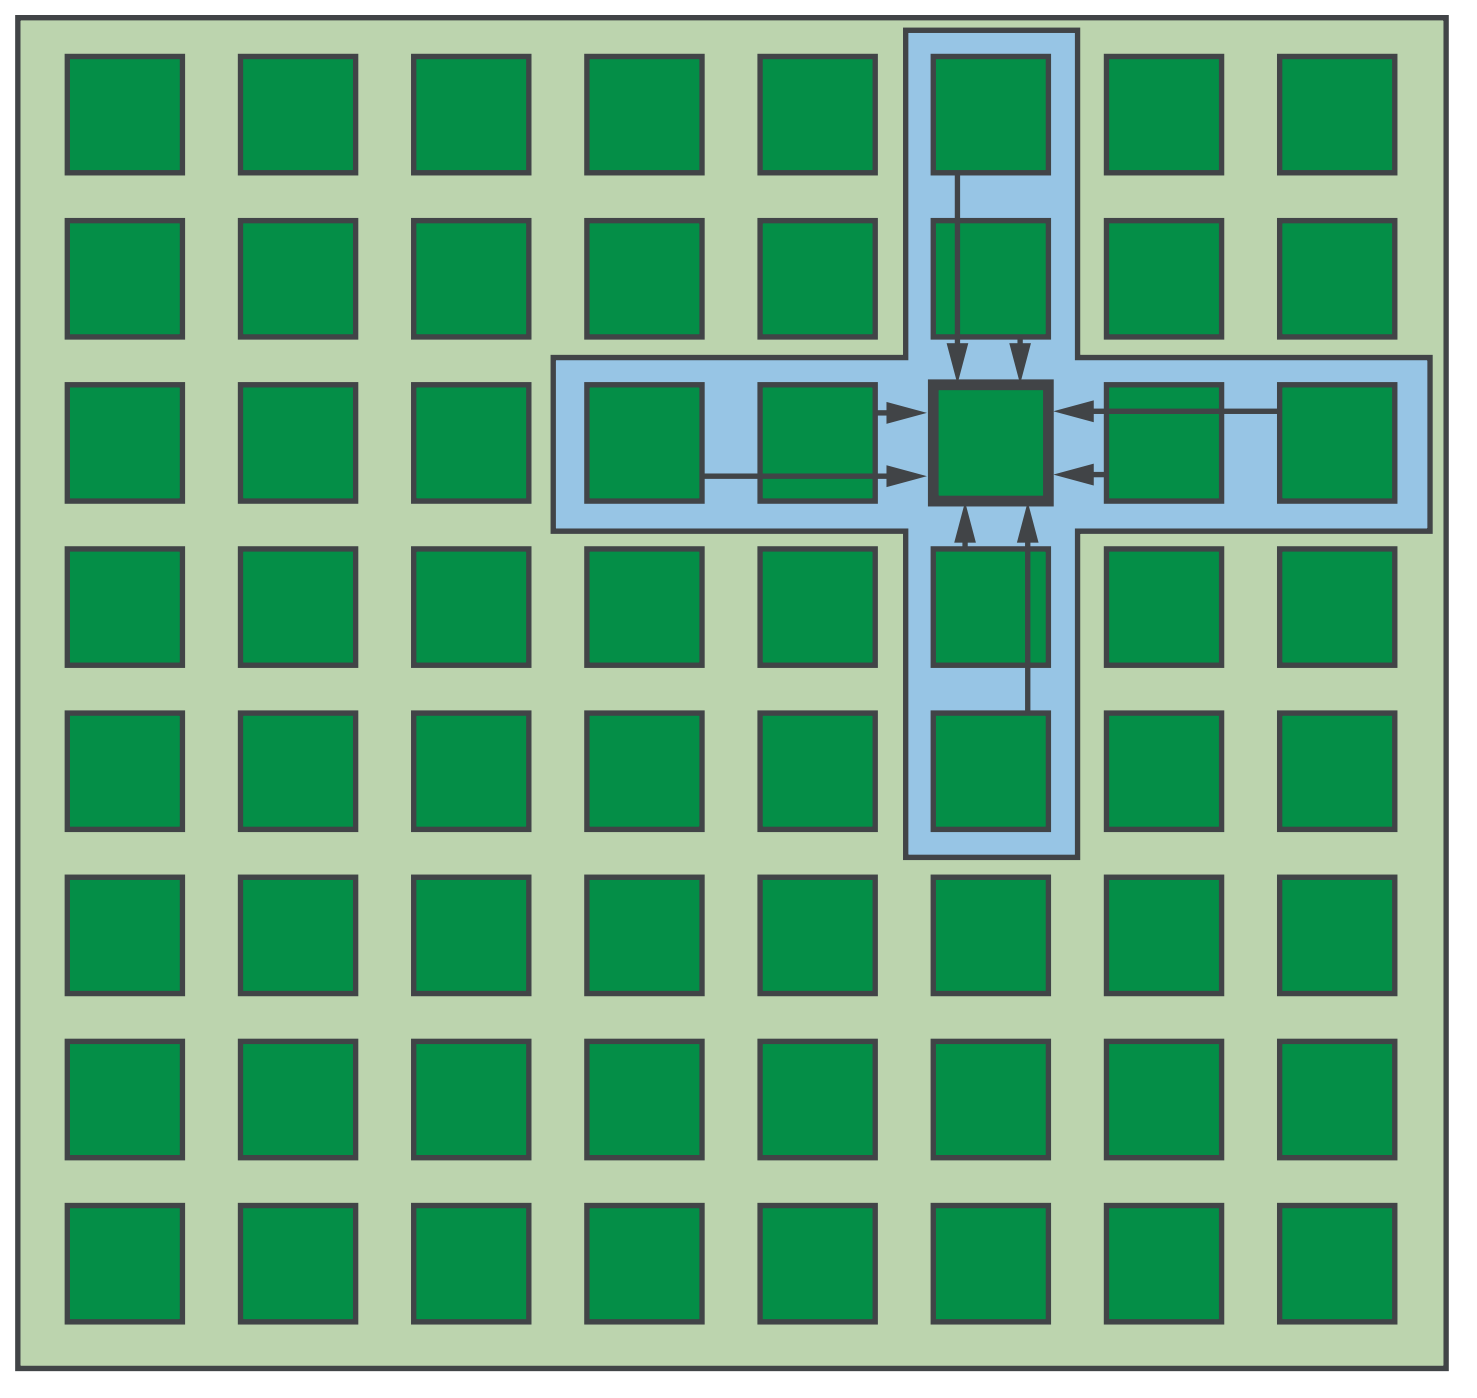
\includegraphics[width=1.\textwidth]{content/chapter-14/images/3}
\end{center}

当模具模式在不同的地方执行时(例如,将输出写入一个单独的存储位置),该函数可以独立地应用于每个输入。现实中调度模板通常比这更复杂:计算相邻的输出需要相同的数据,并且多次从内存中加载该数据会降低性能;我们可能希望就地应用模板(即,重写原始输入值),以减少应用程序的内存占用。\par

因此,模板内核对不同设备的适用性高度依赖于模具的属性和输入。以下有一些经验法则:\par

\begin{itemize}
	\item 小模具可以利用GPU的便笺存储器。
	\item 大型模具可以利用于CPU(相对而言)的缓存。
	\item 通过在FPGA上实现收缩阵列,在小输入上操作的小模板可以获得显著的性能增益。
\end{itemize}

模具很容易描述,但要有效地实现却很复杂,所以模具是领域特定语言(DSL)开发中最活跃的领域之一。已经有一些嵌入式的DSL利用C++的模板元编程能力在编译时生成高性能的模具内核,我们希望这些移植到DPC++上只是时间问题。\par

\hspace*{\fill} \par %插入空行
\textbf{Reduction——归约}

归约模式是一种常见的并行模式,使用典型的关联和交换操作符(例如加法)组合内核调用的每个实例的部分结果。例子是计算一个和(例如,计算一个点积)或计算最小/最大值(例如,使用最大速度来设置时间步长)。\par

\hspace*{\fill} \par %插入空行
图14-4 归约模式
\begin{center}
	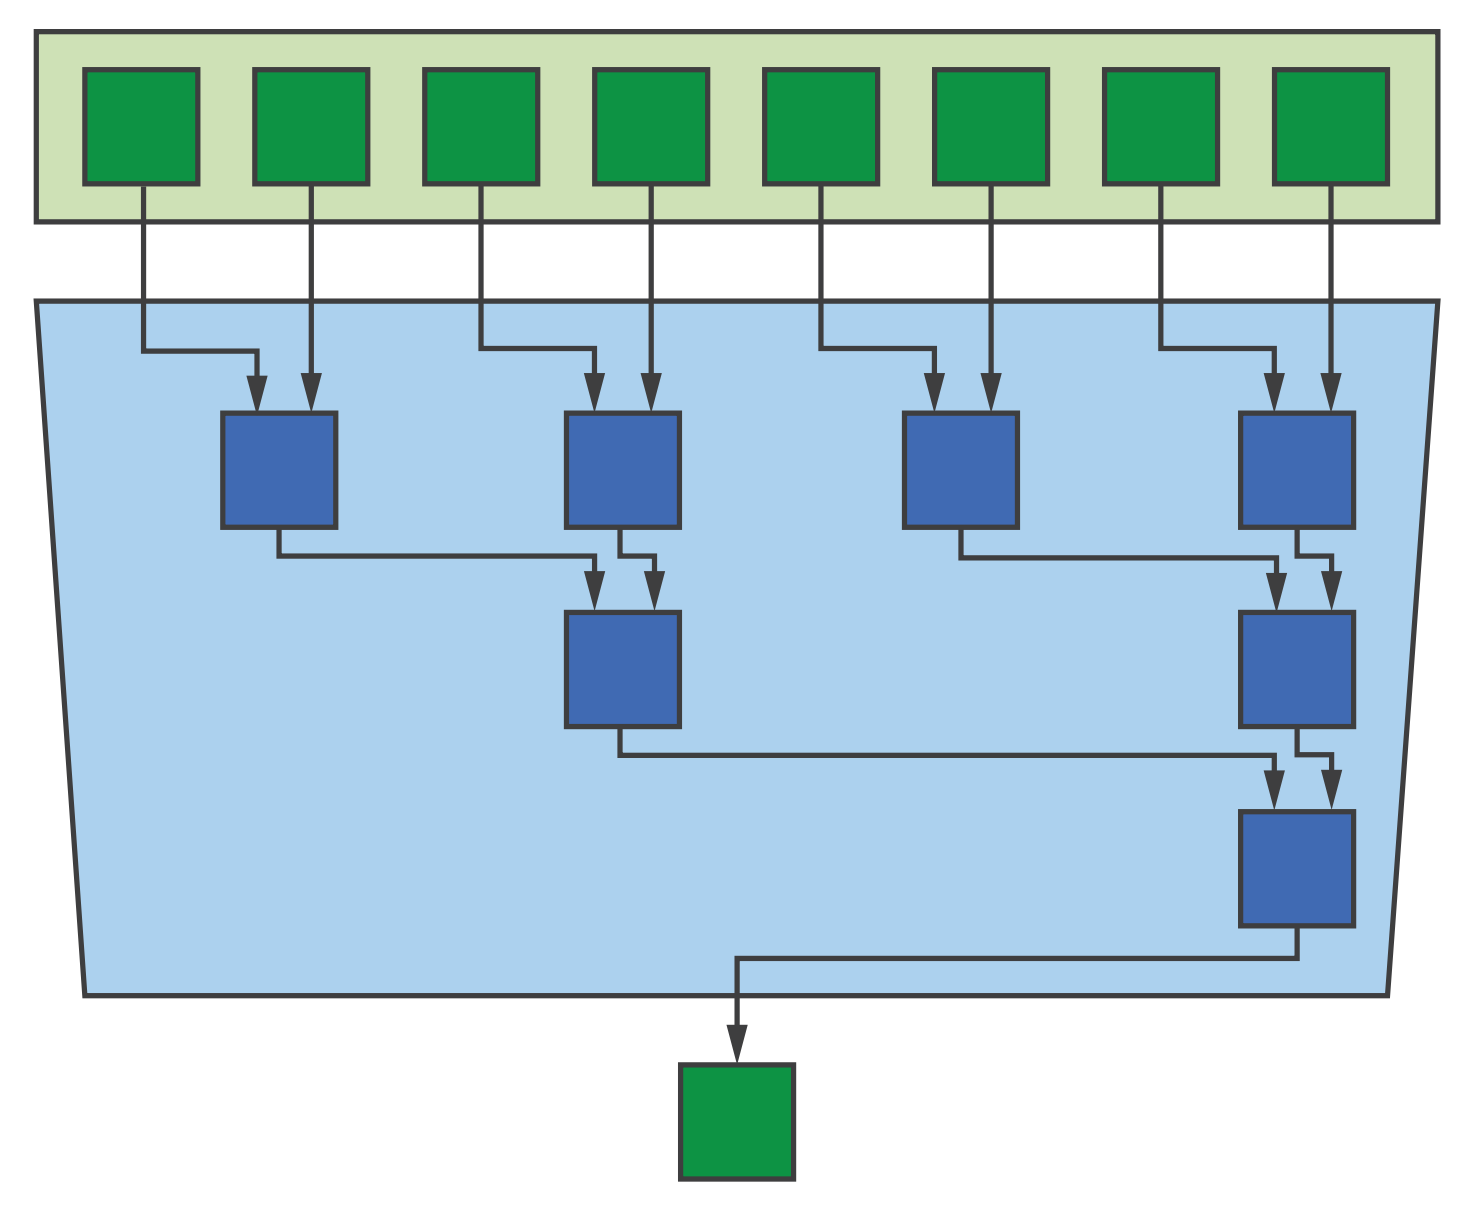
\includegraphics[width=1.\textwidth]{content/chapter-14/images/4}
\end{center}

图14-4显示了通过树归约实现的归约模式,需要对N个输入元素的范围进行log2(N)组合操作。尽管树型归约很常见,但是其他的实现也是可能的——归约一个以特定的顺序组合值。\par

内核间很少会地并行,即使是并行的,也经常与归约(如MapReduce框架)配对。这使得归约成为需要理解的最重要的并行模式之一,也是必须能够在任何设备上有效执行的模式。\par

针对不同设备进行扩展需要进行性能权衡,即计算部分所花费的时间和组合它们所花费的时间。使用过少的并行度会增加计算时间,而使用过多的并行度会增加合并时间。\par

通过使用不同的设备来执行计算和组合步骤,来提高系统的整体利用率可能很不错,但是这种调优工作必须注意在设备之间移动数据的成本。实践中,我们发现在产生数据的同时在同一设备上直接执行数据归约通常是最好的方法。因此,使用多个设备来提高归约模式的性能并不依赖于任务的并行性,而是依赖于另一种级别的数据并行性(即,每个设备对输入数据的一部分执行归约)。\par

\hspace*{\fill} \par %插入空行
\textbf{Scan——扫描}

扫描模式使用二进制关联运算符计算一个广义前缀和,输出的每个元素表示一个部分结果。扫描包容第一个元素,如果元素的部分和的范围在[0,i](即之和(包括i)。扫描排除第一个元素,如果元素的部分和的范围在[0,i])(例如:和不包括i)。\par

乍一看,扫描似乎是一个固有的串行操作,因为每个输出的值取决于前一个输出的值!虽然与其他模式相比,扫描获得并行性的机会确实较少(因此可能伸缩性较差),但图14-5显示了使用对相同数据的多次扫描实现并行扫描是可能的。\par

\hspace*{\fill} \par %插入空行
图14-5 扫描模式
\begin{center}
	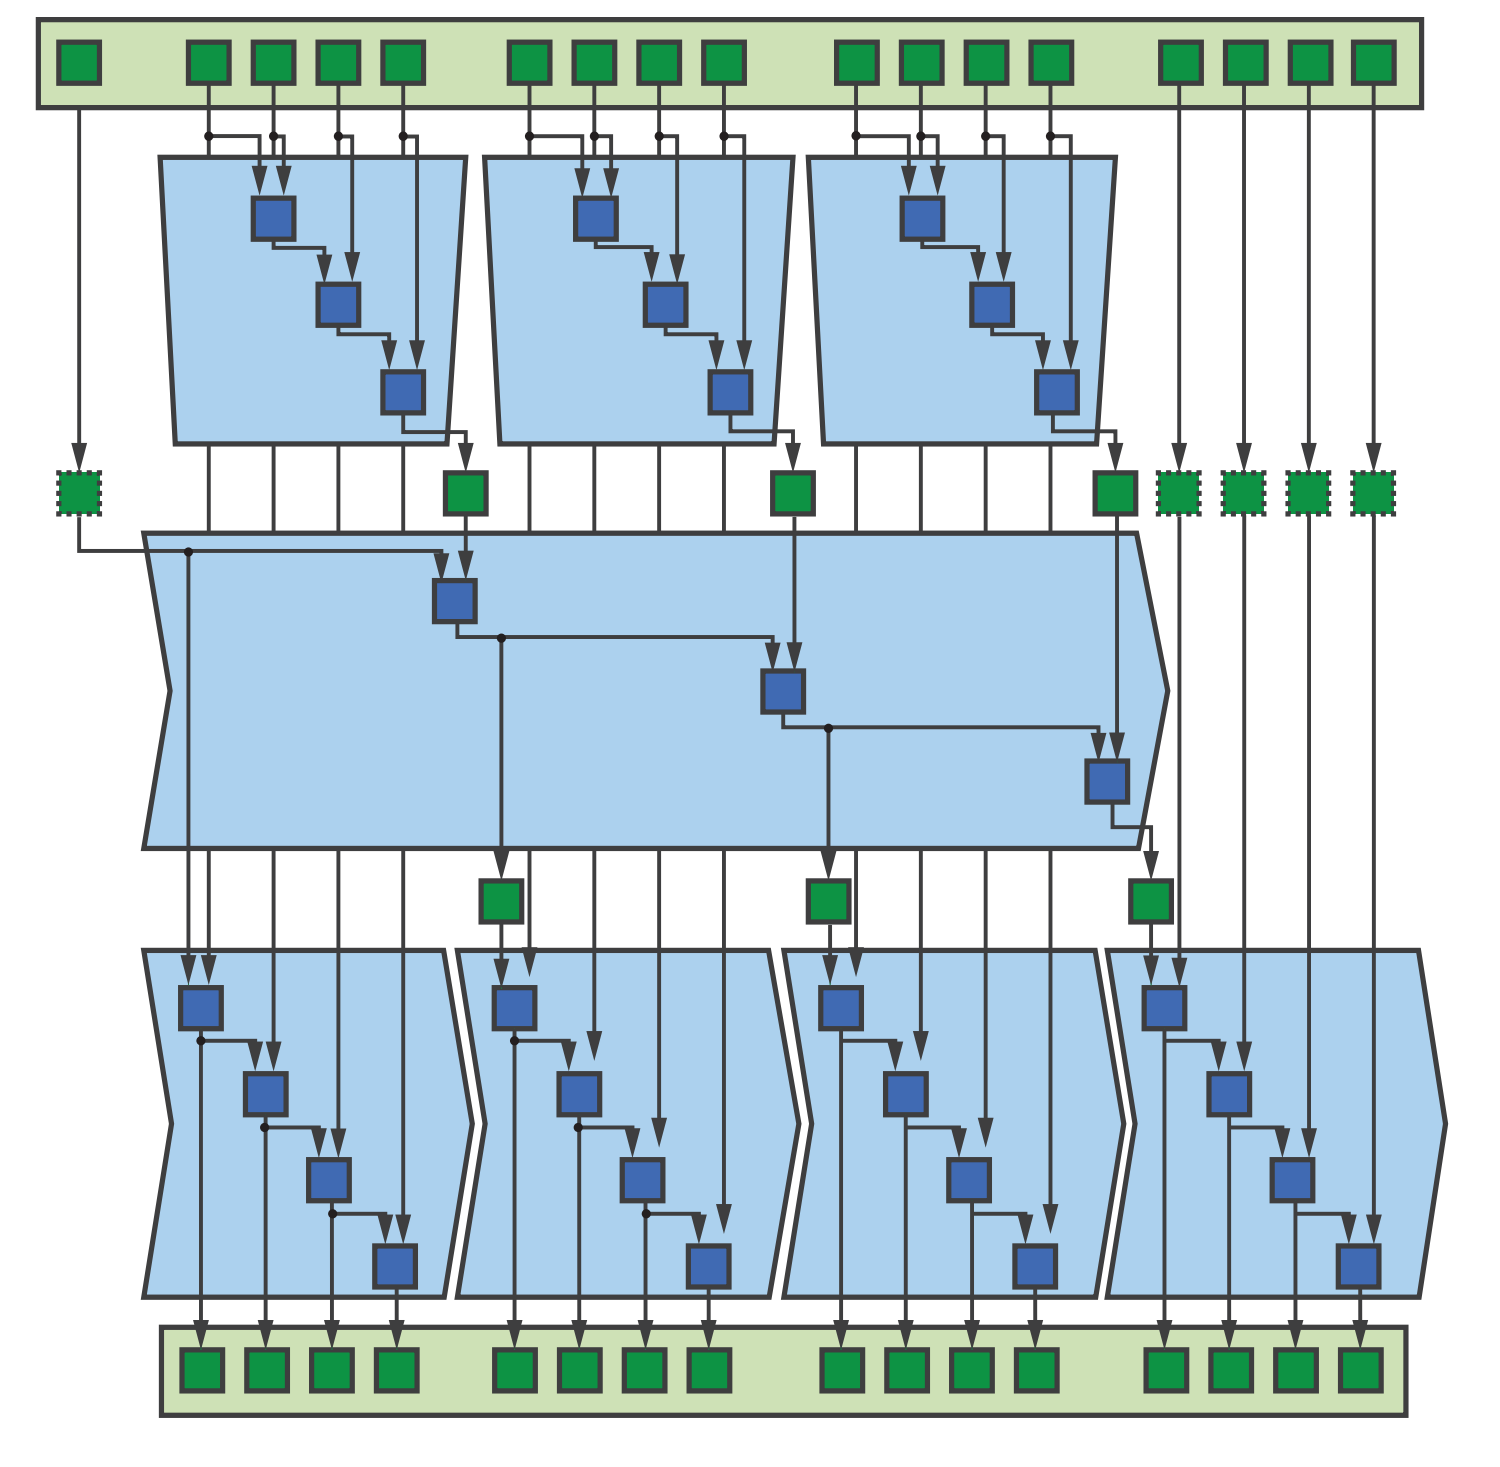
\includegraphics[width=1.\textwidth]{content/chapter-14/images/5}
\end{center}

因为在扫描操作中并行性的机会是有限的,所以执行扫描的最佳设备高度依赖于问题的大小:较小的问题更适合CPU,因为只有较大的问题才会包含足够的数据并行性使GPU饱和。对于FPGA和其他架构来说,问题的大小不太重要,因为扫描本身就有助于管道并行性。处理归约的一个经验法则是,在产生数据的设备上执行扫描操作——考虑在优化期间扫描操作适合应用程序的位置和方式——通常会比专注于单独优化扫描操作产生更好的结果。\par

\hspace*{\fill} \par %插入空行
\textbf{打包和解包}

打包和解包模式与扫描密切相关,通常在扫描功能的基础上实现。在这里单独讨论,因为它们是常见操作(例如,添加到列表)的高性能实现,这些操作可能与求前缀和没有明显的联系。\par

\hspace*{\fill} \par %插入空行
\textbf{打包}

打包模式,如图14-6所示,基于布尔条件丢弃输入范围中的元素,将未丢弃的元素打包到输出范围的连续位置。这个布尔条件可以是预先计算的掩码,也可以通过对每个输入元素应用某个函数在线计算。\par

\hspace*{\fill} \par %插入空行
图14-6 打包模式
\begin{center}
	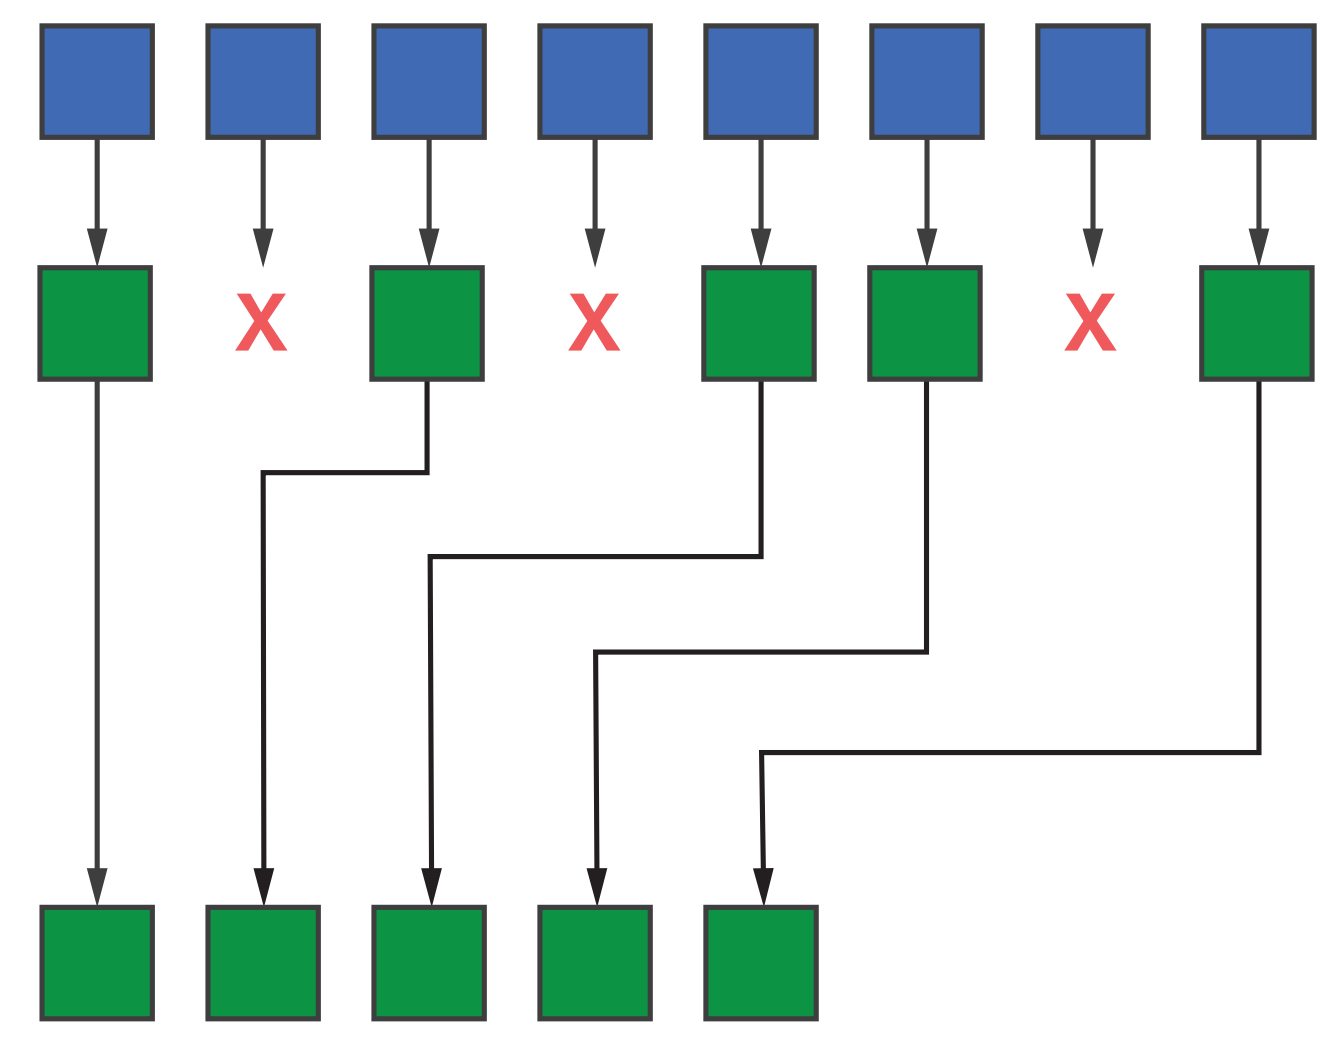
\includegraphics[width=1.\textwidth]{content/chapter-14/images/6}
\end{center}

与扫描一样,打包操作具有串行性。给定要打包/复制的输入元素,计算在输出范围中的位置需要关于有多少先前的元素也打包/复制到输出中的信息。这个信息相当于对布尔条件的独占性扫描。\par

\hspace*{\fill} \par %插入空行
\textbf{解包}

如图14-7所示(顾名思义),解包模式与打包模式相反。输入范围内的连续元素被解包为输出范围内的非连续元素,而不影响其他元素。这个模式最明显的用例是解包以前打包的数据,也可以用来填充以前计算产生的数据中的“空白”。\par

\hspace*{\fill} \par %插入空行
图14-7 解包模式
\begin{center}
	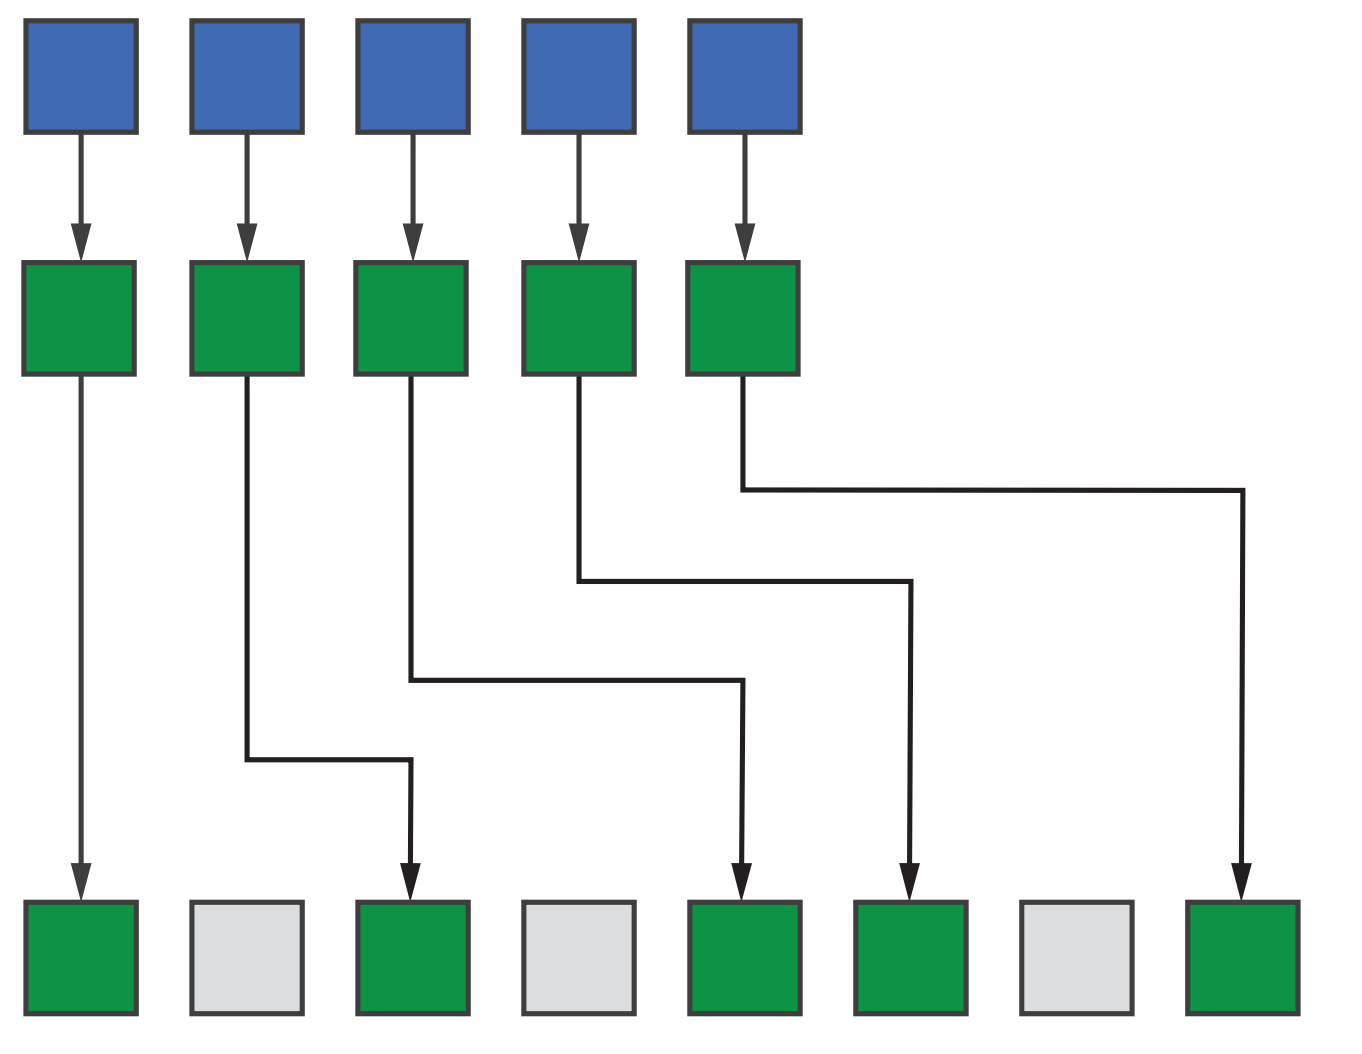
\includegraphics[width=1.\textwidth]{content/chapter-14/images/7}
\end{center}


















